\chapter{Fundamentação Teórica}

\section{Funcionamento do coração}
\label{sec:funciionamento_coracao}

O coração é um órgão muscular composto por quatro câmaras — átrio direito e esquerdo, e ventrículo direito e esquerdo — que se contraem de forma rítmica, bombeando sangue para o corpo. Essas contrações são controladas por correntes elétricas que percorrem o coração de maneira precisa e em velocidade controlada.

Na figura \ref{fig:coracao_esquema_eletrico}, o sistema de condução elétrico do coração é ilustrado.

\begin{figure}[H]
  \centering
  \caption{Sistema de condução do coração}
   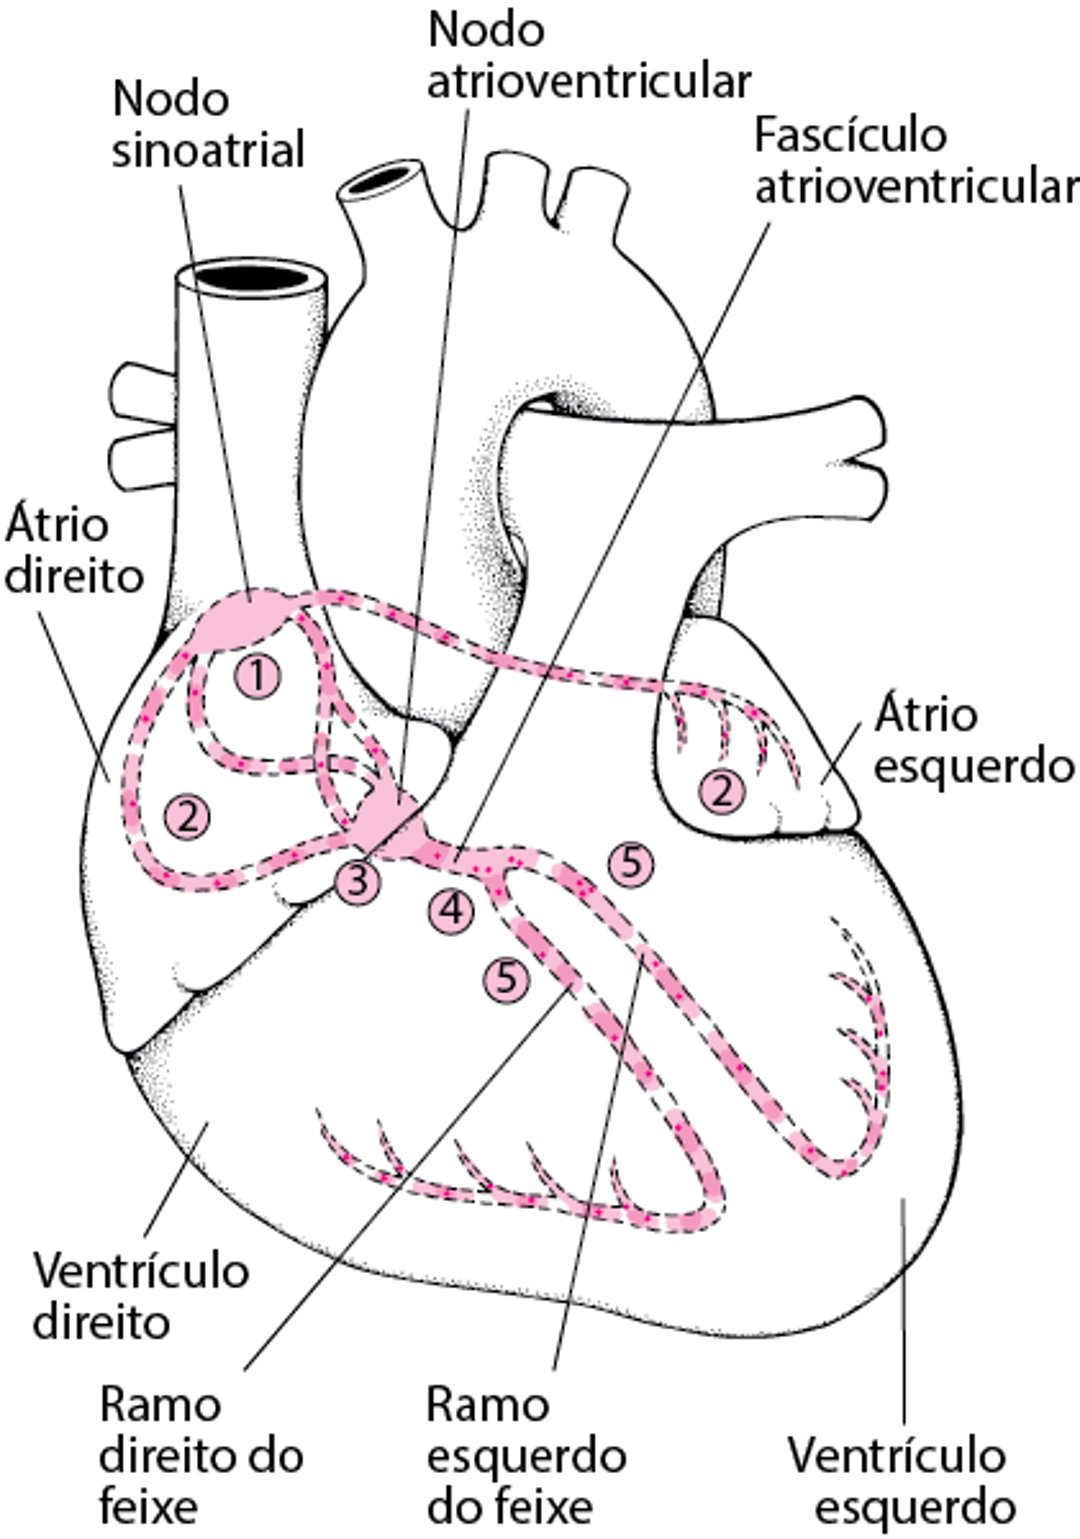
\includegraphics[width=0.6\textwidth]{figuras/coracao_sistema_eletrico.png} % insere o tikzpicture puro
  \label{fig:coracao_esquema_eletrico}
    \legend{Fonte: Adaptado de \citeonline{Mitchell_Arritmias_MSD}}
\end{figure}

Segundo \citeonline{Mitchell_Arritmias_MSD}, o batimento cardíaco normal se inicia no nódulo sinusal (1), localizado no átrio direito, que atua como o marcapasso natural do coração. A corrente elétrica propaga-se do átrio direito para o esquerdo (2), promovendo sua contração e o bombeamento do sangue para os ventrículos. Em seguida, o impulso atinge o nódulo atrioventricular (3) — conexão entre os átrios e ventrículos — onde é temporariamente retardado, permitindo que os átrios se contraiam completamente e encham as câmaras inferiores.

Posteriormente, a corrente percorre o feixe de His (4), que se divide e conduz o impulso para ambos os ventrículos (5), promovendo sua contração e o bombeamento do sangue para o restante do corpo.

\section{O eletrocardiograma}
\label{sec:ecg}

O eletrocardiograma, ECG, é um enxame não invasivo usado para medir a atividade elétrica do coração. Ele é feito a partir do contato de eletrodos, chamados de derivações ou \textit{leads}, sobre a pele.
A quantidade de eletrodos varia, mas geralmente são 12 \cite{msd_ecg}.

Ao registrar a magnitude e direção da corrente, as derivações geram uma onda que representa a atividade elétrica do coração. O passo a passo descrito em \ref{sec:funciionamento_coracao} é refletido em sua morfologia.

Na figura \ref{fig:ecg_exemplo_coracao}, um  ECG de um batimento, observe que ele é subdividido em: onda P, complexo QRS e onda T \cite{msd_ecg}. Note que cada uma dessas partes se refere a um estágio do batimento.

\begin{figure}[H]
  \centering
  \caption{Exemplo de ECG com sua morfologia destacada}
   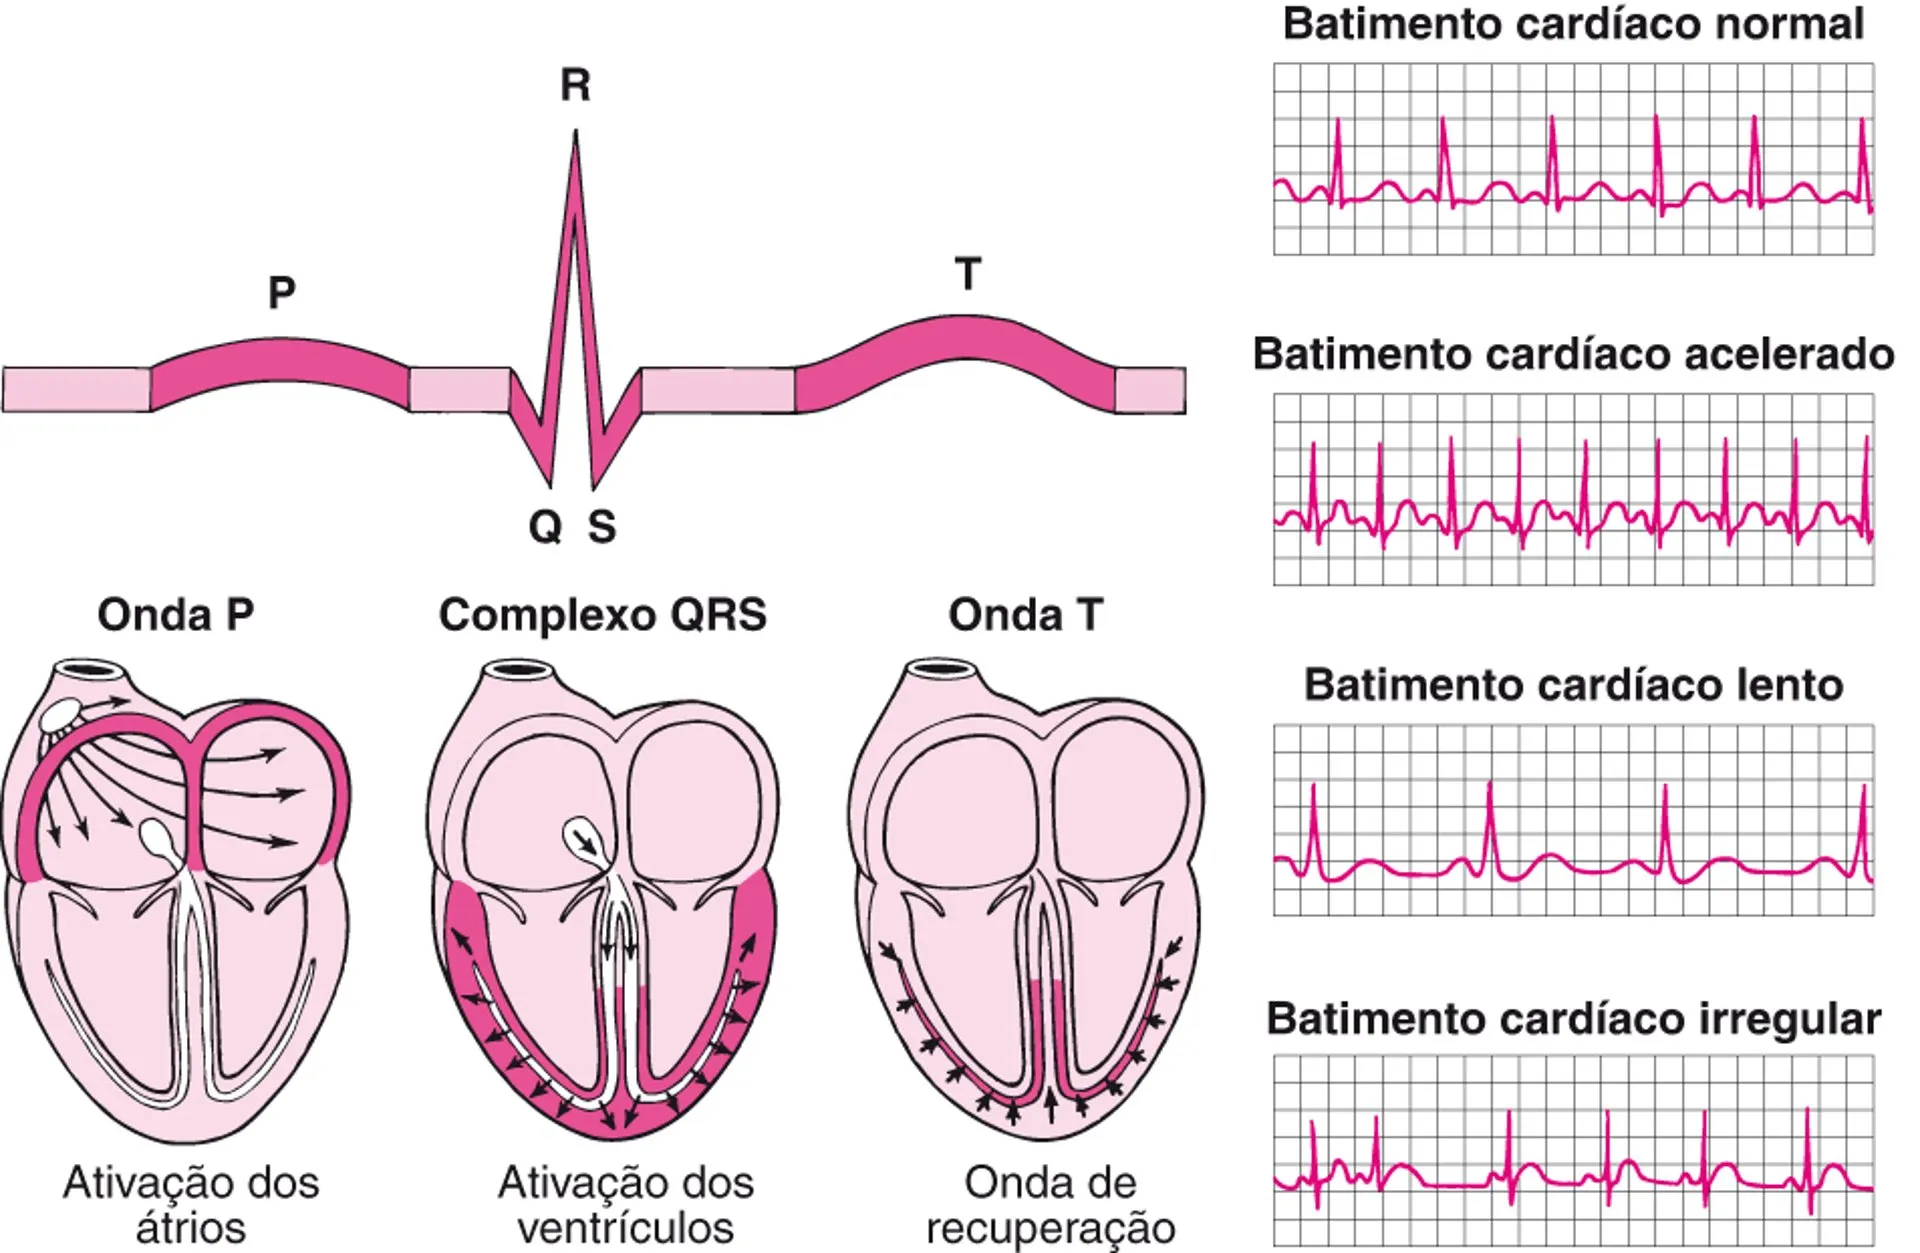
\includegraphics[width=0.8\textwidth]{figuras/ecg_exemplo_coracao.png} % insere o tikzpicture puro
  \label{fig:ecg_exemplo_coracao}
    \legend{Fonte: Adaptado de  \citeonline{msd_ecg}}
\end{figure}

Dentre as doenças que podem ser diagnósticas via ECG estão as arritmias cardíacas. 

\section{Arritmias}


\subsection{Arritmias clínicas}

As arritmias são alterações no ritmo cardíaco que podem ter diversas causas, incluindo alterações hormonais, uso de medicamentos, toxinas (como álcool ou cafeína), anomalias eletrolíticas ou doenças cardíacas.
Segundo \citeonline{Mitchell_Arritmias_MSD}, em adultos em repouso, a frequência cardíaca normal varia entre 60 e 100 batimentos por minuto (bpm). Frequências mais baixas, conhecidas como bradicardia sinusal, são comuns em atletas, crianças pequenas, adolescentes, jovens adultos e durante o sono. Por outro lado, a taquicardia sinusal ocorre quando a frequência se eleva, podendo ser observada durante o esforço físico, doenças, estimulação neural simpática ou emoção intensa.

Variações no ritmo cardíaco são fenômenos fisiológicos normais. Durante a respiração, por exemplo, é comum que a frequência aumente e diminua levemente — comportamento conhecido como arritmia sinusal respiratória. O autor ainda observa que um ritmo cardíaco perfeitamente regular pode indicar patologias no sistema nervoso autônomo, como ocorre em casos de diabetes avançado. Dessa forma, ainda não existe um indicador global e definitivo do que seria um ritmo sinusal considerado saudável.
As arritmias podem ser classificadas de forma simplificada em três tipos principais:

\begin{enumerate}
    \item Taquicardia: frequência excessivamente rápida;
    \item Bradicardia: frequência excessivamente lenta;
    \item Irregular: quando os impulsos percorrem o coração por vias irregulares.
\end{enumerate}

\subsection{Padrões de classificação para algoritmos (AAMI)}

A AAMI define cinco classes de arritmia; normal (N), ventricular (V), superventricular (S), fusão (F) e não classificado (Q) \cite{silva2025,saadatnejad2020}.


